\documentclass[a4paper,12pt]{article}
\usepackage[pdftex, hidelinks]{hyperref}

\usepackage{bm}
\usepackage[T1]{fontenc}
\usepackage[utf8]{inputenc}
\usepackage{algorithmic}
\usepackage{algorithm}
\usepackage{amsfonts}
\usepackage{amssymb}
\usepackage{courier}
\usepackage{booktabs}
\usepackage{graphicx}
\usepackage{listings}
\usepackage{mathtools}
\usepackage{amssymb}
\lstset{basicstyle=\footnotesize\ttfamily,
        breakatwhitespace = false,
        breaklines = true,
        keepspaces = true,
        language = R,
        showspaces = false,
        showstringspaces = false,
        belowcaptionskip = \bigskipamount,
        framerule = 0.80pt,
        frame = tb,
        belowskip = \bigskipamount,
        escapeinside={<@}{@>}}

\title{TDDE01 -- Machine Learning \\
       Group 9 Laboration Report 4}
\author{{Martin Estgren \texttt{<mares480>}} \\
        {Erik S. V. Jansson \texttt{<erija578>}} \\
        {Sebastian Maghsoudi \texttt{<sebma654>}} \\~\\
        {Linköping University (LiU), Sweden}}

\begin{document}

    \pagenumbering{arabic}
    \maketitle % Generate.

    \section*{Assignment 1}

        This assignment involves examining a given data set called \emph{State}, which contains the observations about the \emph{population} \& \emph{economy} in different \emph{states}. We are primarily interested in the relationship between the \emph{metropolitan habitation rate (MET)} and the \emph{public expenditure per capita (EX)} for a state.

    \subsection*{Raw Data Analysis}

        We first analyze the data by plotting the \emph{EX} target as a function of \emph{MET}. These results can be observed in the plotted Figure~\ref{fig:state}, notice the spread of data.

        \begin{figure}[H]
            \centering
            \caption{Plot of Metropolitan Rate \& Expenditure}
            \label{fig:state}
            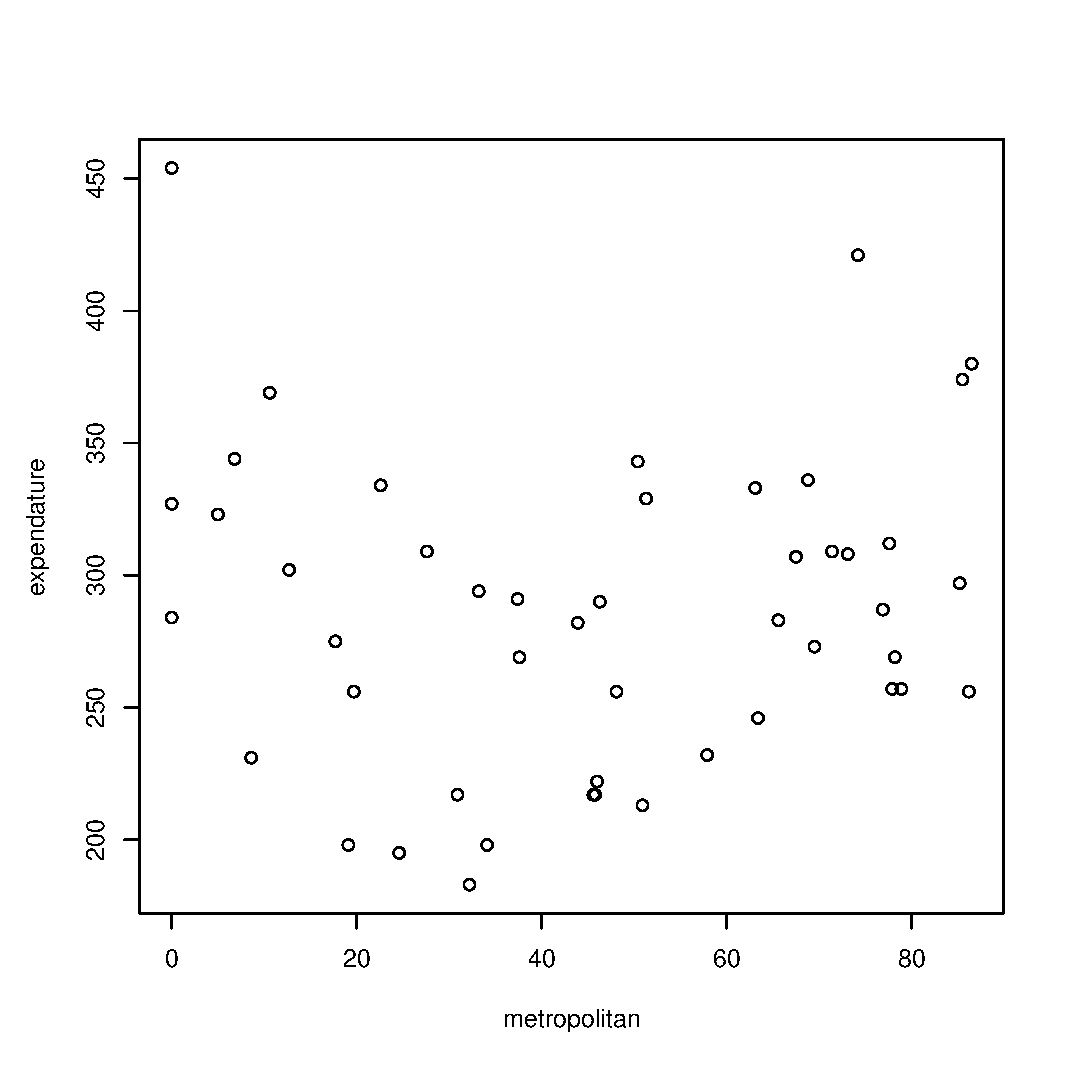
\includegraphics[width=\textwidth]{share/A1_data.eps}
        \end{figure}

        The figure indicates that a linear model isn't suitable for predicting the target in this data set, no easily visible pattern can be observed in this plot. Since we are tasked with using \emph{regression trees} in this assignment, the first step is to fit such a model with it, then finding the optimal number of leaves.

    \subsection*{Regression Tree Analysis}

        We have examined how a \emph{regression tree model} fits the data set using \emph{cross-validation} for finding the optimal number of \emph{leaves}. The plotted \emph{decision tree} from the fitted model can be seen in Figure~\ref{fig:tree}. This model was fitted with the following piece of \emph{R} code:

        \lstinputlisting[firstline=9,lastline=14]{../share/assignment1.r}

        \begin{figure}[H]
            \centering
            \caption{Plotted Decision Tree for Model}
            \label{fig:tree}
            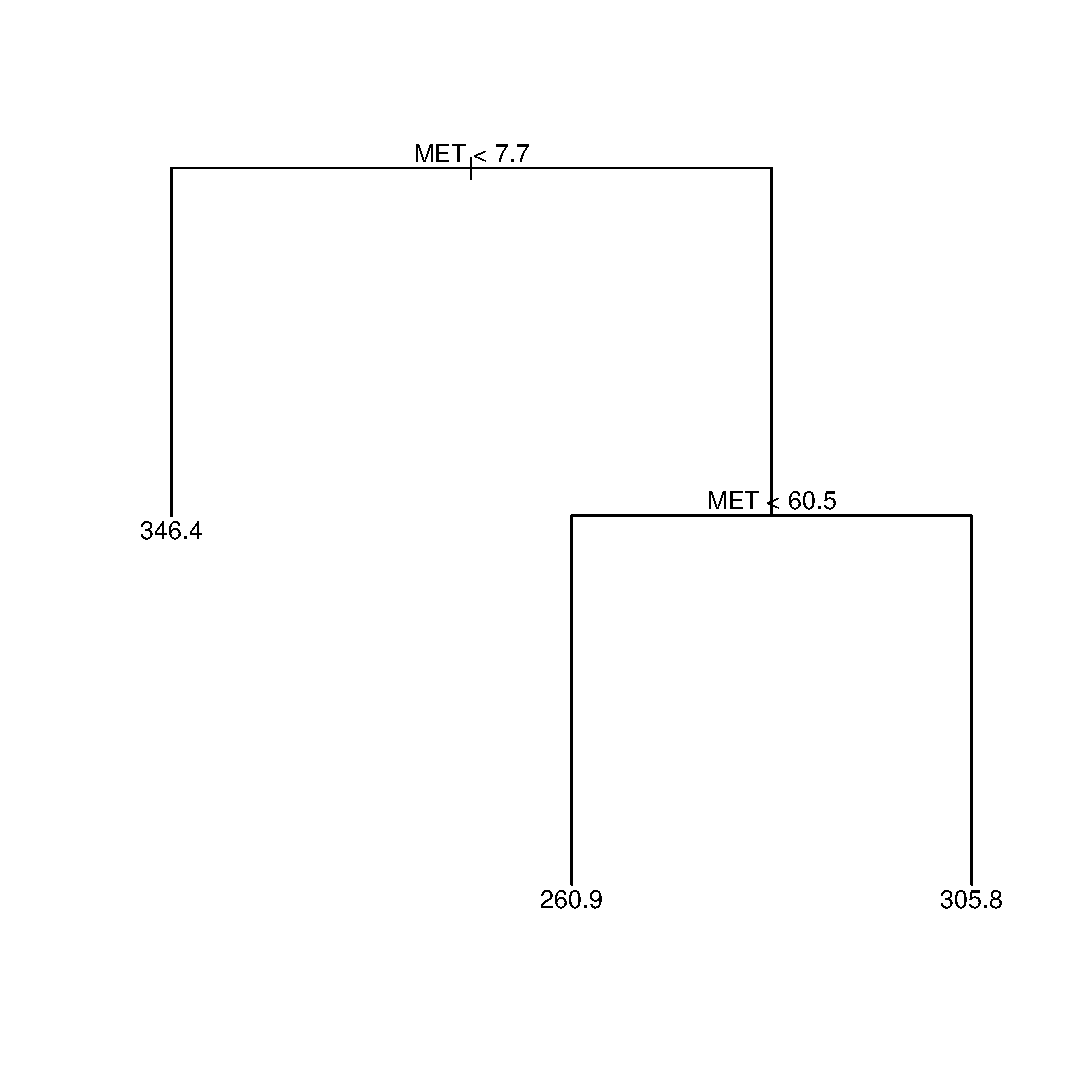
\includegraphics[width=\textwidth]{share/A1_tree.eps}
        \end{figure}

        According to the cross-validation, the optimal number of leaves is 3, which we use to prune the full tree model and get the best optimal model. These predicted results of the best model can be seen in Figure~\ref{fig:predicted}.

        \begin{figure}[H]
            \centering
            \caption{Plot of Metropolitan Rate \& Predict Ex}
            \label{fig:predicted}
            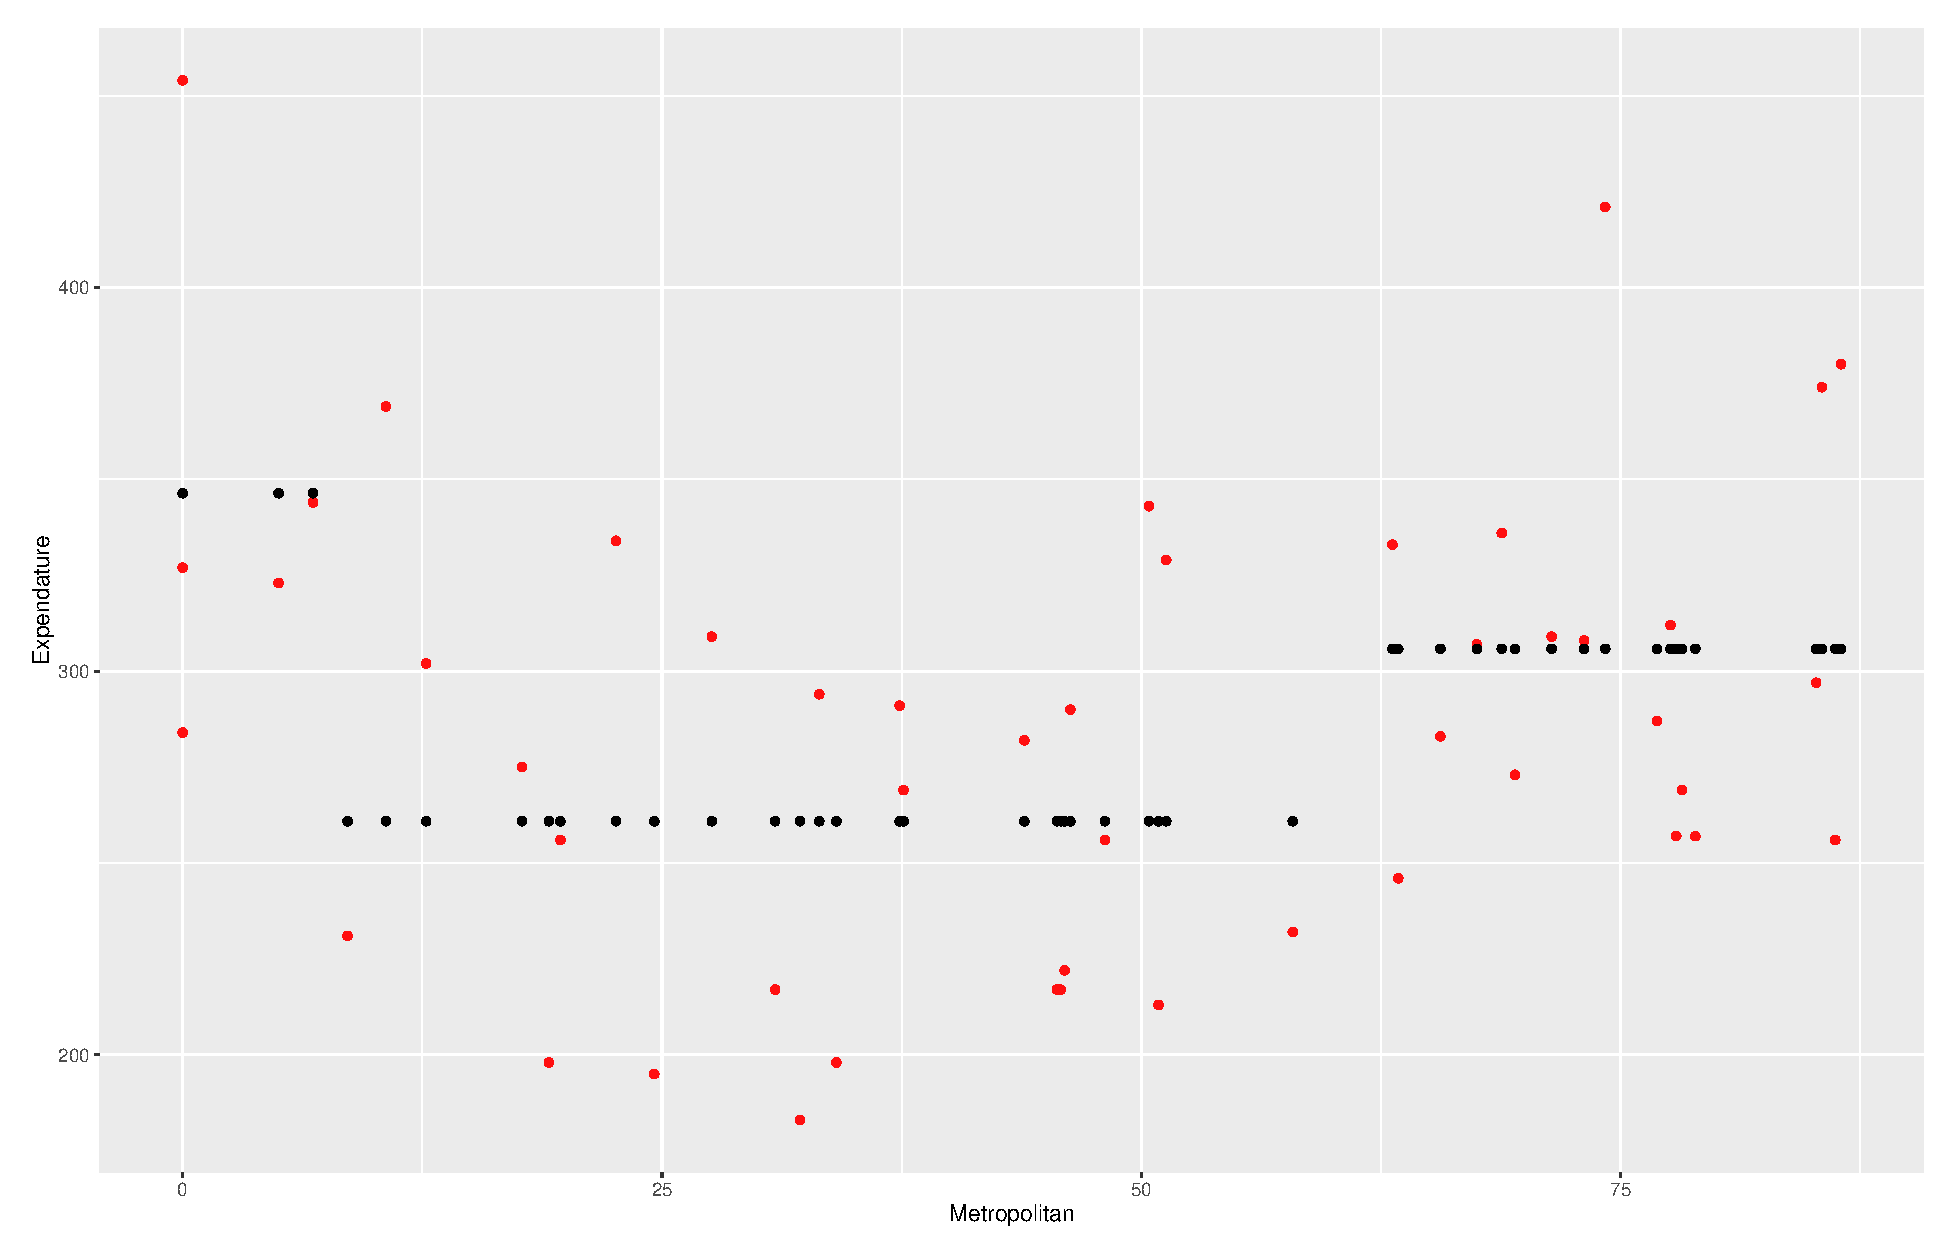
\includegraphics[width=\textwidth]{share/A1_fit.eps}
        \end{figure}

        Notice how the above results indicate that the predictions (black) have produced less labels than the original data (in red). These correspond to the three resulting leaves derived from cross-validation. Also, each label is roughly located around the mean of the raw data (that has been divided in ``buckets'').

        Finally, the frequency of the model's residuals are displayed in the Figure~\ref{fig:residuals} below, derived by using:

        \lstinputlisting[firstline=22,lastline=22]{../share/assignment1.r}

        \begin{figure}[H]
            \centering
            \caption{Histogram of the Residuals}
            \label{fig:residuals}
            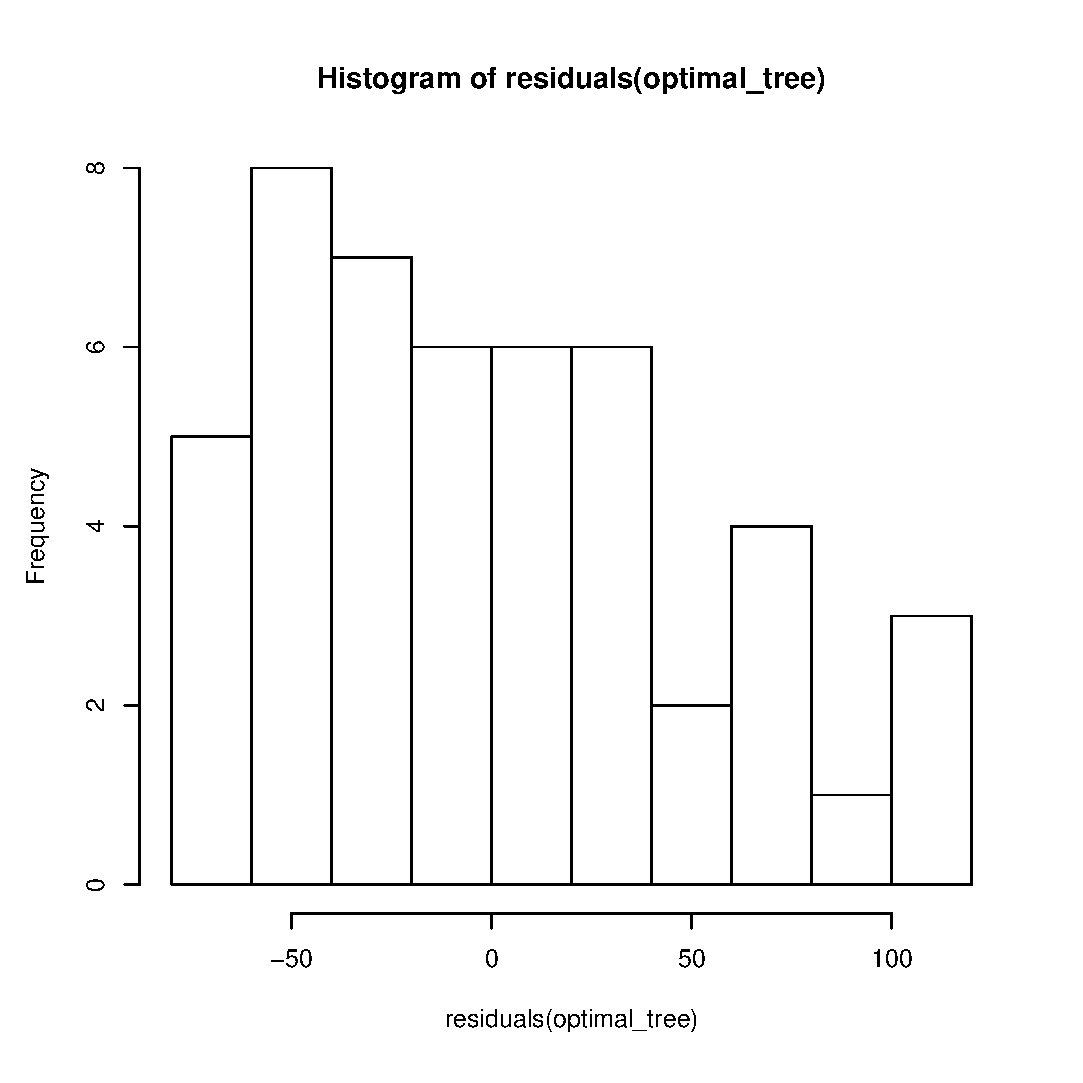
\includegraphics[width=\textwidth]{share/A1_historgram_residuals.eps}
        \end{figure}

        Preferably, the above distribution should be a \emph{bell curve} around 0, meaning predictions weren't good.

    \subsection*{Non-Parametric Bootstrap}

        We explore the same data set as before, still being modeled with a \emph{regression tree model} using the \emph{non-parametric bootstrap}. \emph{Bootstrapping} is used to estimate the properties of an estimator by sampling from an approximated distribution. In the case of \emph{non-parametric bootstrapping}, the underlying distribution is assumed to \emph{not} be known, and the data is instead re-sampled with replacement. The estimated distribution is then given by $\hat{f}(D_1), \hat{f}(D_2), ..., \hat{f}(D_B)$, estimator $\hat{f}$ and data $D_i$.

        For our data set, we re-sample 1000 times using the \emph{non-parametric bootstrapping} function \texttt{boot}, for a confidence level of 95 \% (which is an $\alpha = 5\%$). By retrieving the \emph{confidence intervals} for each $x_i$ and plotting them, we get the \emph{confidence bands} of the model. Which can be seen in a Figure~\ref{fig:confidence_bands} below. Listing~\ref{lst:assignment1} does the \emph{non-parametric bootstrapping} in:

        \lstinputlisting[firstline=25,lastline=34]{../share/assignment1.r}

        \begin{figure}[H]
            \centering
            \caption{Confidence Bands of Regression Tree with non-parametric bootstrap}
            \label{fig:confidence_bands}
            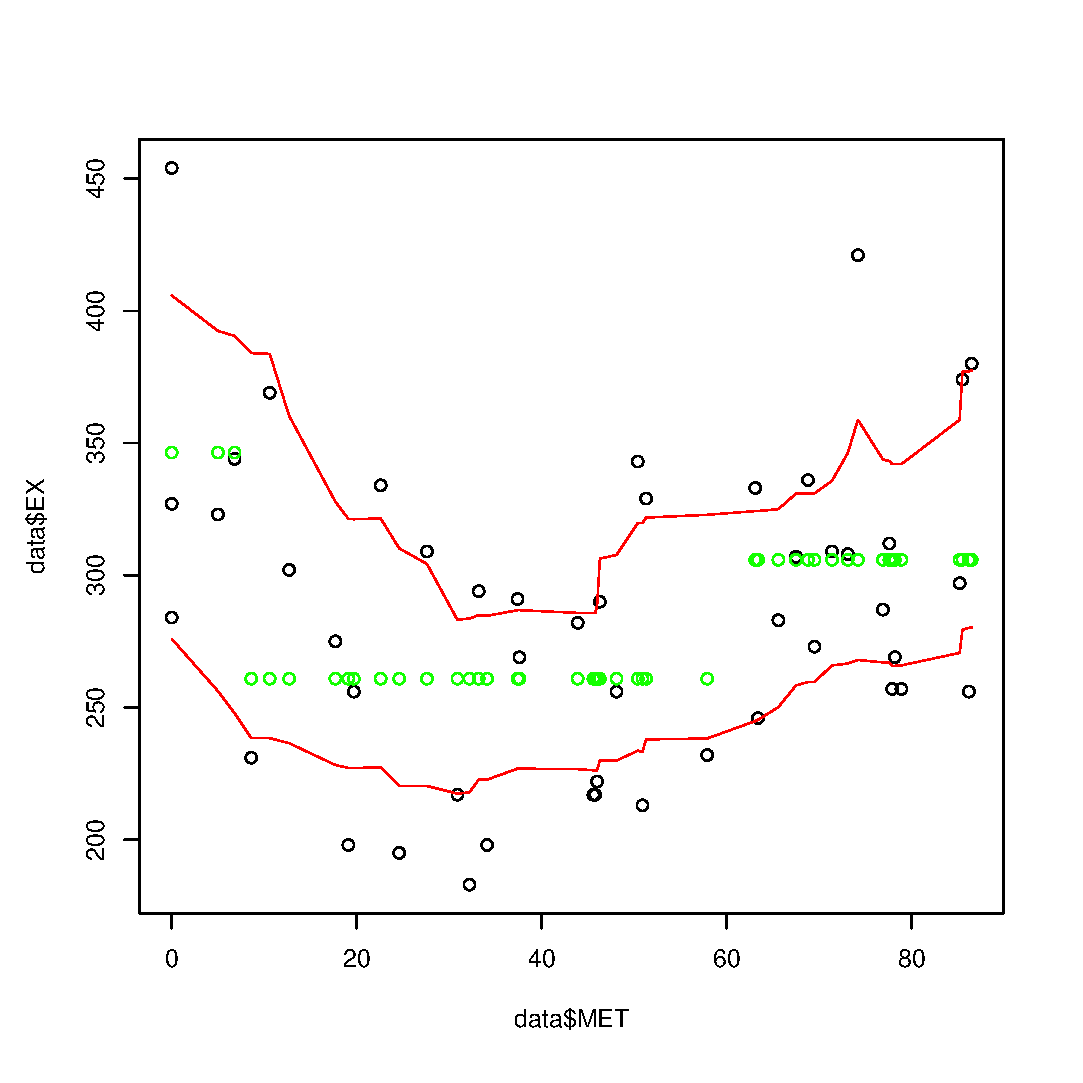
\includegraphics[width=\textwidth]{share/A1_nonparametric.eps}
        \end{figure}

        Notice how several observations are outside the confidence band derived from our regression tree model.

    \subsection*{Parametric Bootstrap}

        Now the preconditions have changed as opposed to the \emph{non-parametric bootstrap}, since the underlying distribution is now ``known'' to be: $Y \sim \mathcal{N}(\mu_i, \sigma^2)$. Having the distribution allows us to sample from it, giving us the concept of \emph{parametric bootstrapping}. Similarly, the number of samples to be taken into consideration has been chosen to be 1000 again, with a confidence level of 95 \%. Plotting the confidence and prediction bands using \emph{parametric bootstrap} gives Figure~\ref{fig:confpred_bands}. The ``tighter'' band is the \emph{confidence band} while the more relaxed one is the \emph{prediction band}. The following \emph{R} source produces this:
        \lstinputlisting[firstline=51,lastline=56]{../share/assignment1.r}

        \lstinputlisting[firstline=58,lastline=64]{../share/assignment1.r}

        \lstinputlisting[firstline=66,lastline=70]{../share/assignment1.r}

        \lstinputlisting[firstline=72,lastline=75]{../share/assignment1.r}

        \begin{figure}[H]
            \centering
            \caption{Confidence/Prediction Bands Regression the Tree with parametric bootstrap}
            \label{fig:confpred_bands}
            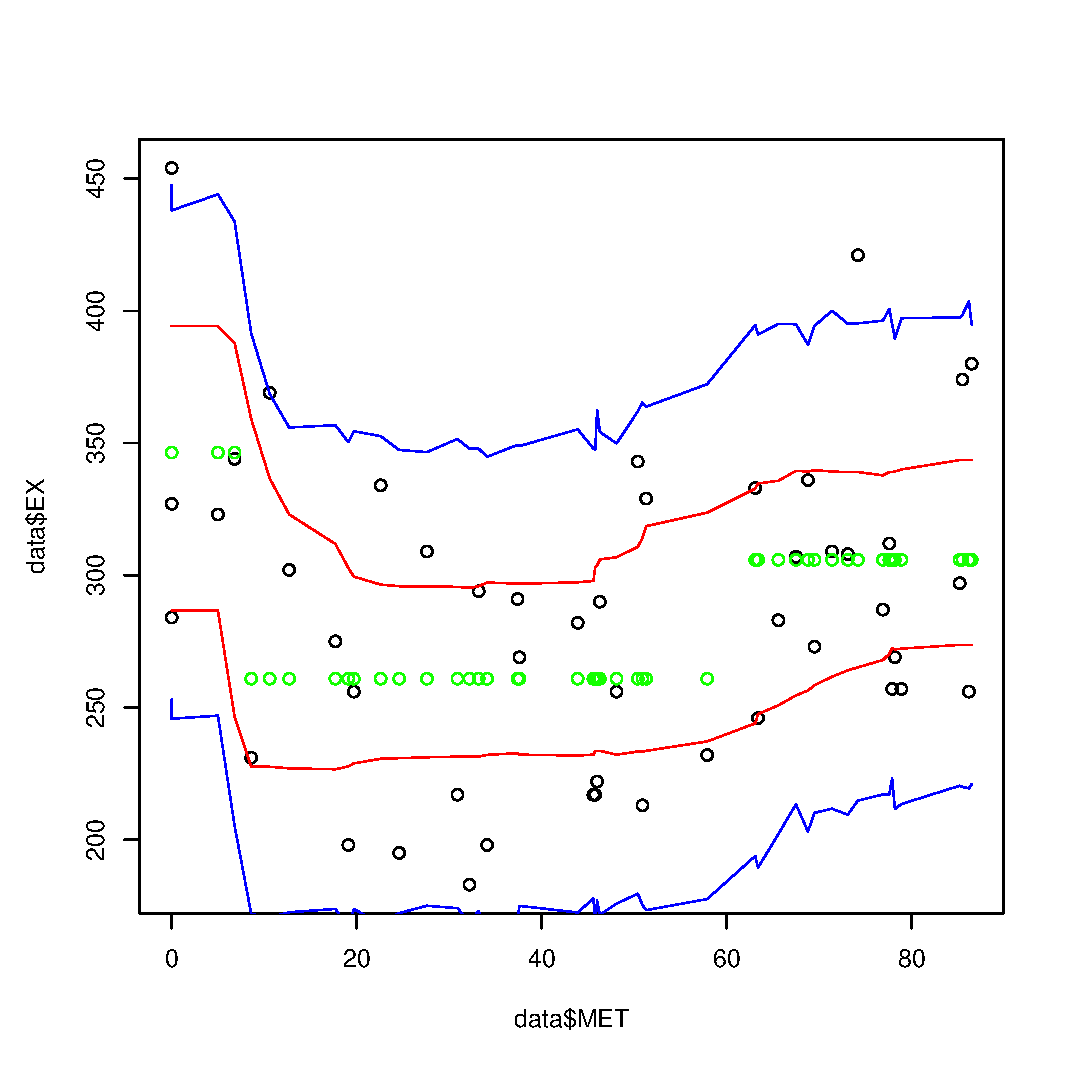
\includegraphics[width=\textwidth]{share/A1_parametric.eps}
        \end{figure}

        As can be noted in the figure above, there are a couple of observations outside the prediction band. This is caused because of the $95 \%$ level of confidence imposed on the prediction band. It seems reasonable that $5 \%$ is outside the prediction band. However, this tells us that our model predicts $95 \%$ of the data correctly, which seems a bit unrealistic. By referring back to the residual histogram, the assumption that the data is normally distributed is a bit of a stretch, at least given the current data set. \emph{Non-parametric bootstrapping} seems more suitable.

        % As can be seen in the figure, there are a pair of observations outside the prediction band. This is of course the result of using $95\%$ confidence.

    \section*{Assignment 2}

        In this assignment we are tasked with analyzing a data set containing observations regarding different levels of \emph{viscosity} and \emph{near-infrared spectra} for many different \emph{diesel fuels} using \emph{PCA} and \emph{ICA} (\emph{Component Analysis Functions}).

    \subsection*{Principal Component Analysis}

        \emph{Principal Component Analysis (PCA)} is used to reduce the number of dimensions in a data set by analyzing the variance that each feature contributes to the distribution. We conduct a PCA on the given data set, this gives us the histogram in Figure~\ref{fig:pcahist}. The R code responsible:

        \lstinputlisting[firstline=6,lastline=10]{../share/assignment2.r}

        \begin{figure}[H]
            \centering
            \caption{PCA histogram of variance}
            \label{fig:pcahist}
            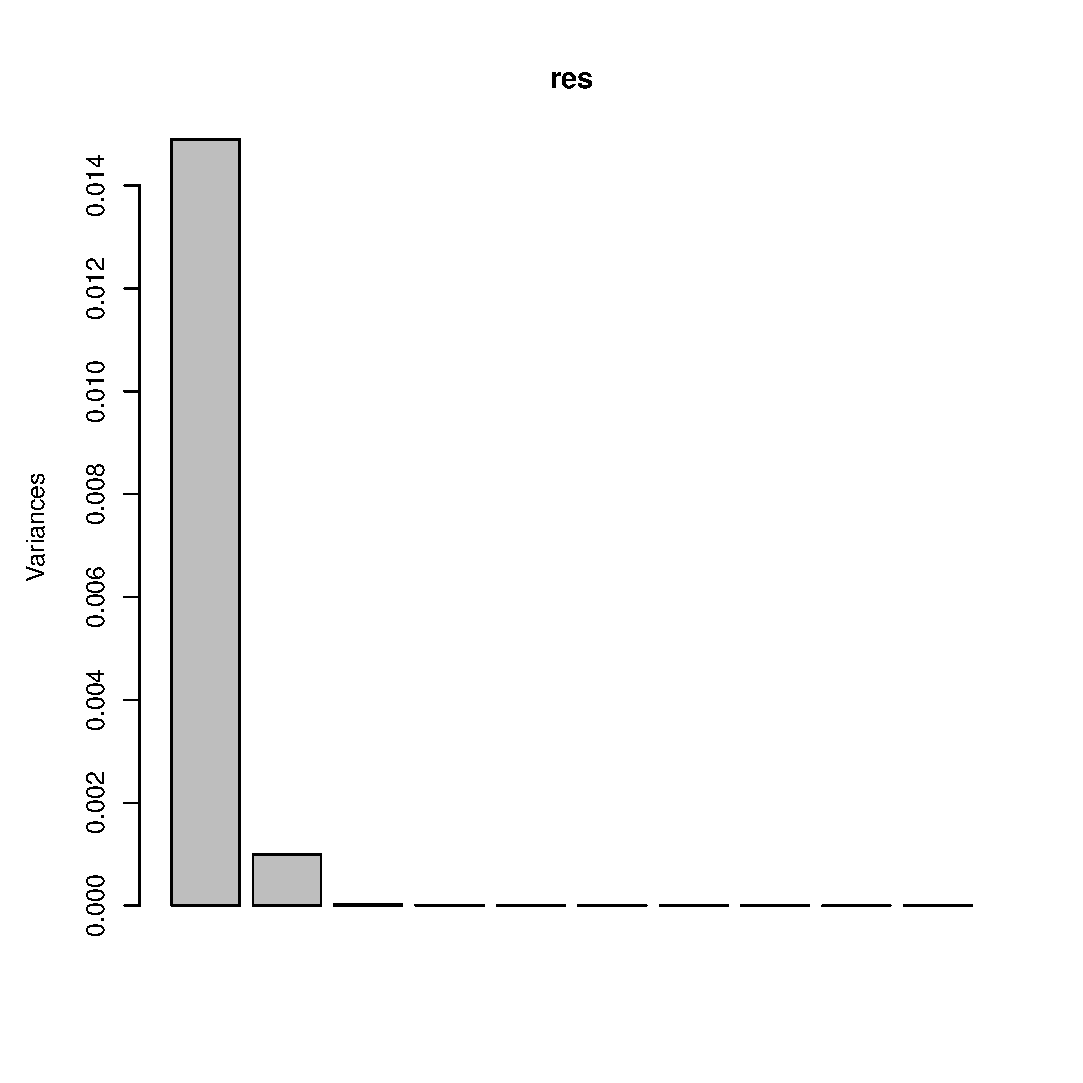
\includegraphics[width=\textwidth]{share/A2_pcahist.eps}
        \end{figure}

        We observe that only two components are required to reach 99 \% cumulative variance, which are \emph{X750 (PC1)} and \emph{X752 (PC2)}. Afterwards, we plot the scores of the chosen principal components in Figure~\ref{fig:pcascore}.

        \begin{figure}[H]
            \centering
            \caption{PCA score distribution}
            \label{fig:pcascore}
            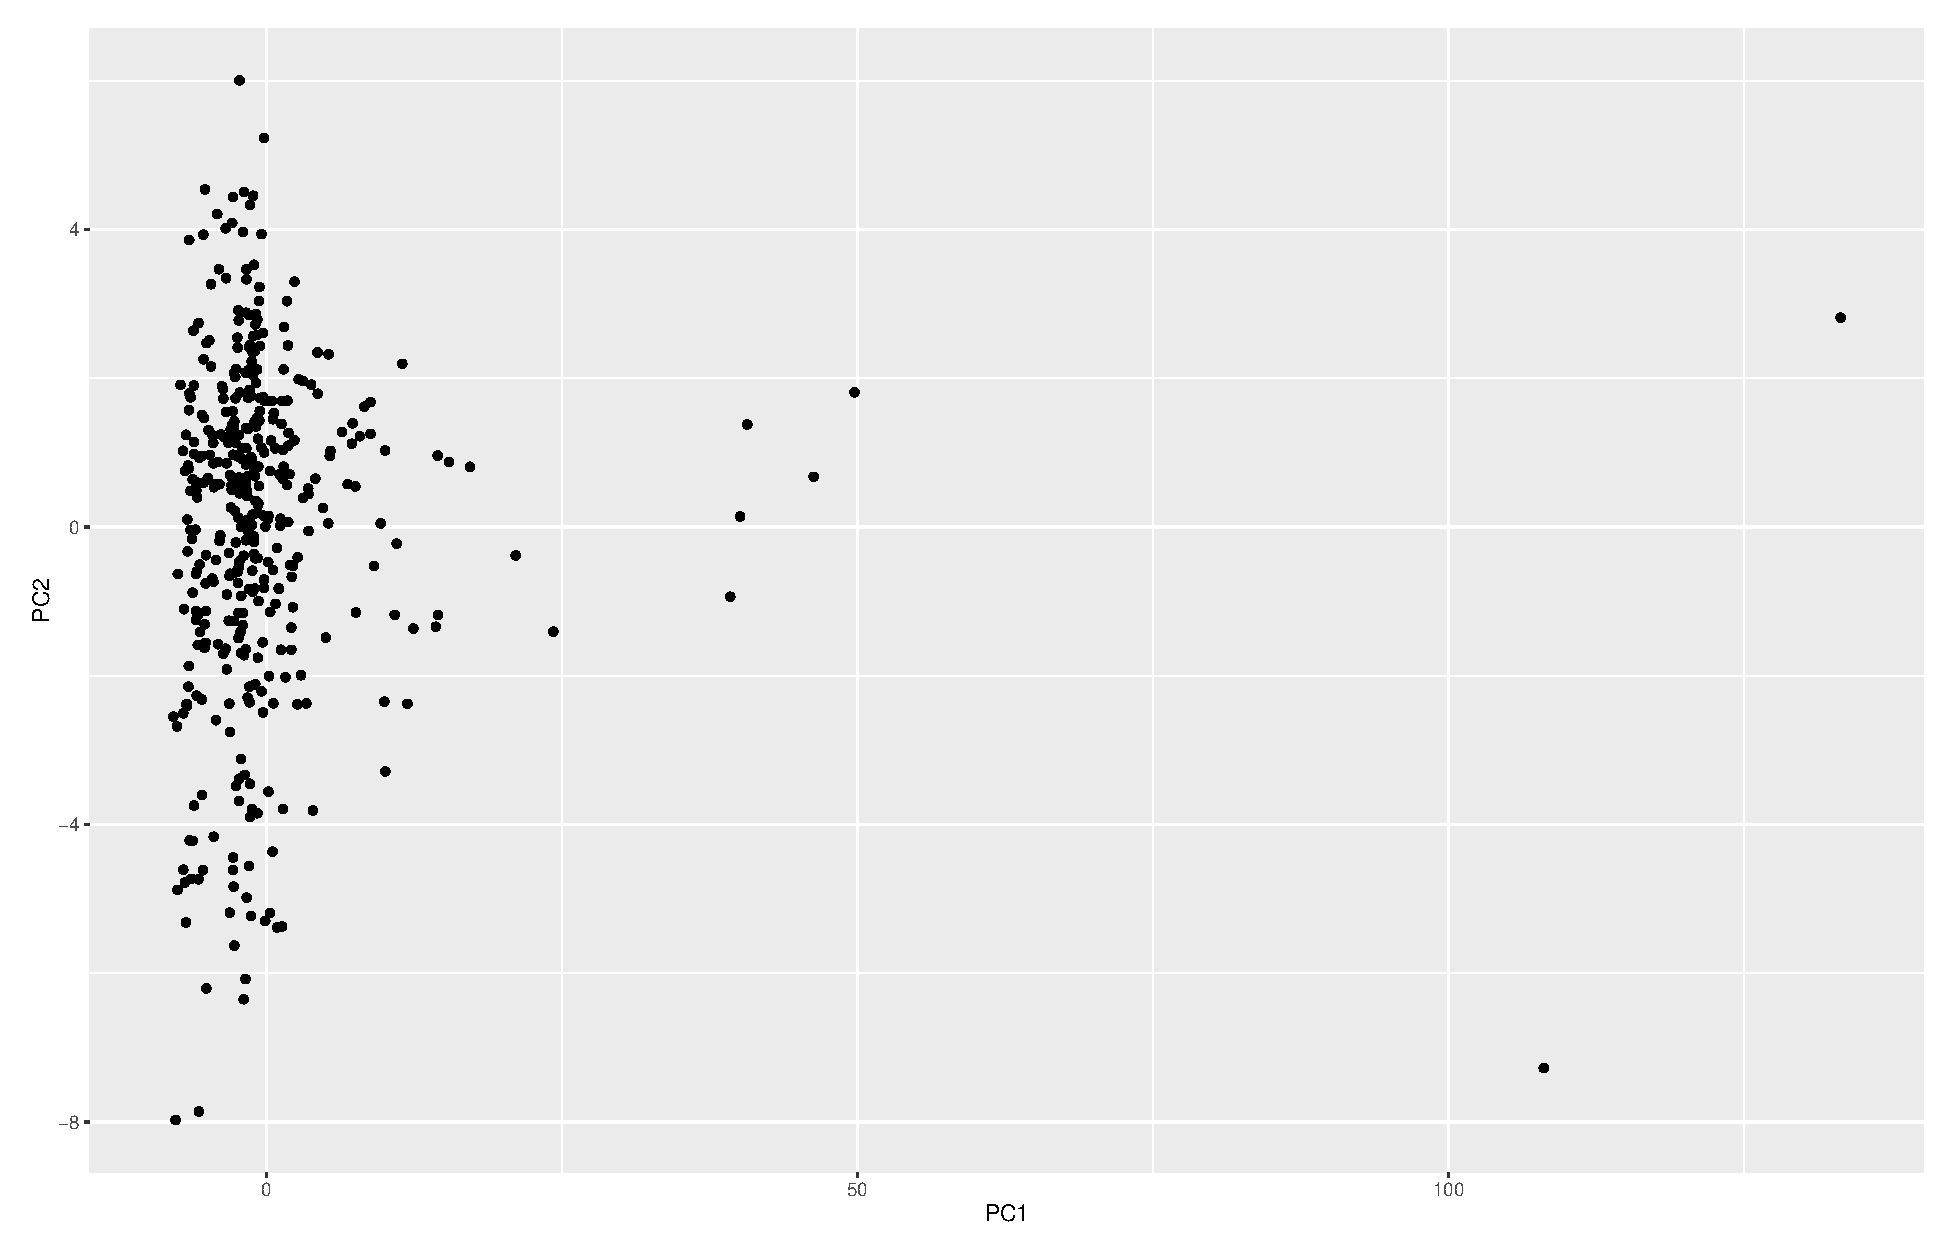
\includegraphics[width=\textwidth]{share/A2_pcascore.eps}
        \end{figure}

        As can be seen, there is a large amount of independence between these two components. The outliers indicates unusual diesel fuels. Now we plot the loadings, which indicates the correlation between components through proportional variance. This is done in Figures~\ref{fig:x750tp}, \ref{fig:x752tp}. 

        \begin{figure}[H]
            \centering
            \begin{minipage}[]{0.49\textwidth}
                \caption{Trace plot of PC1\label{fig:x750tp}}
                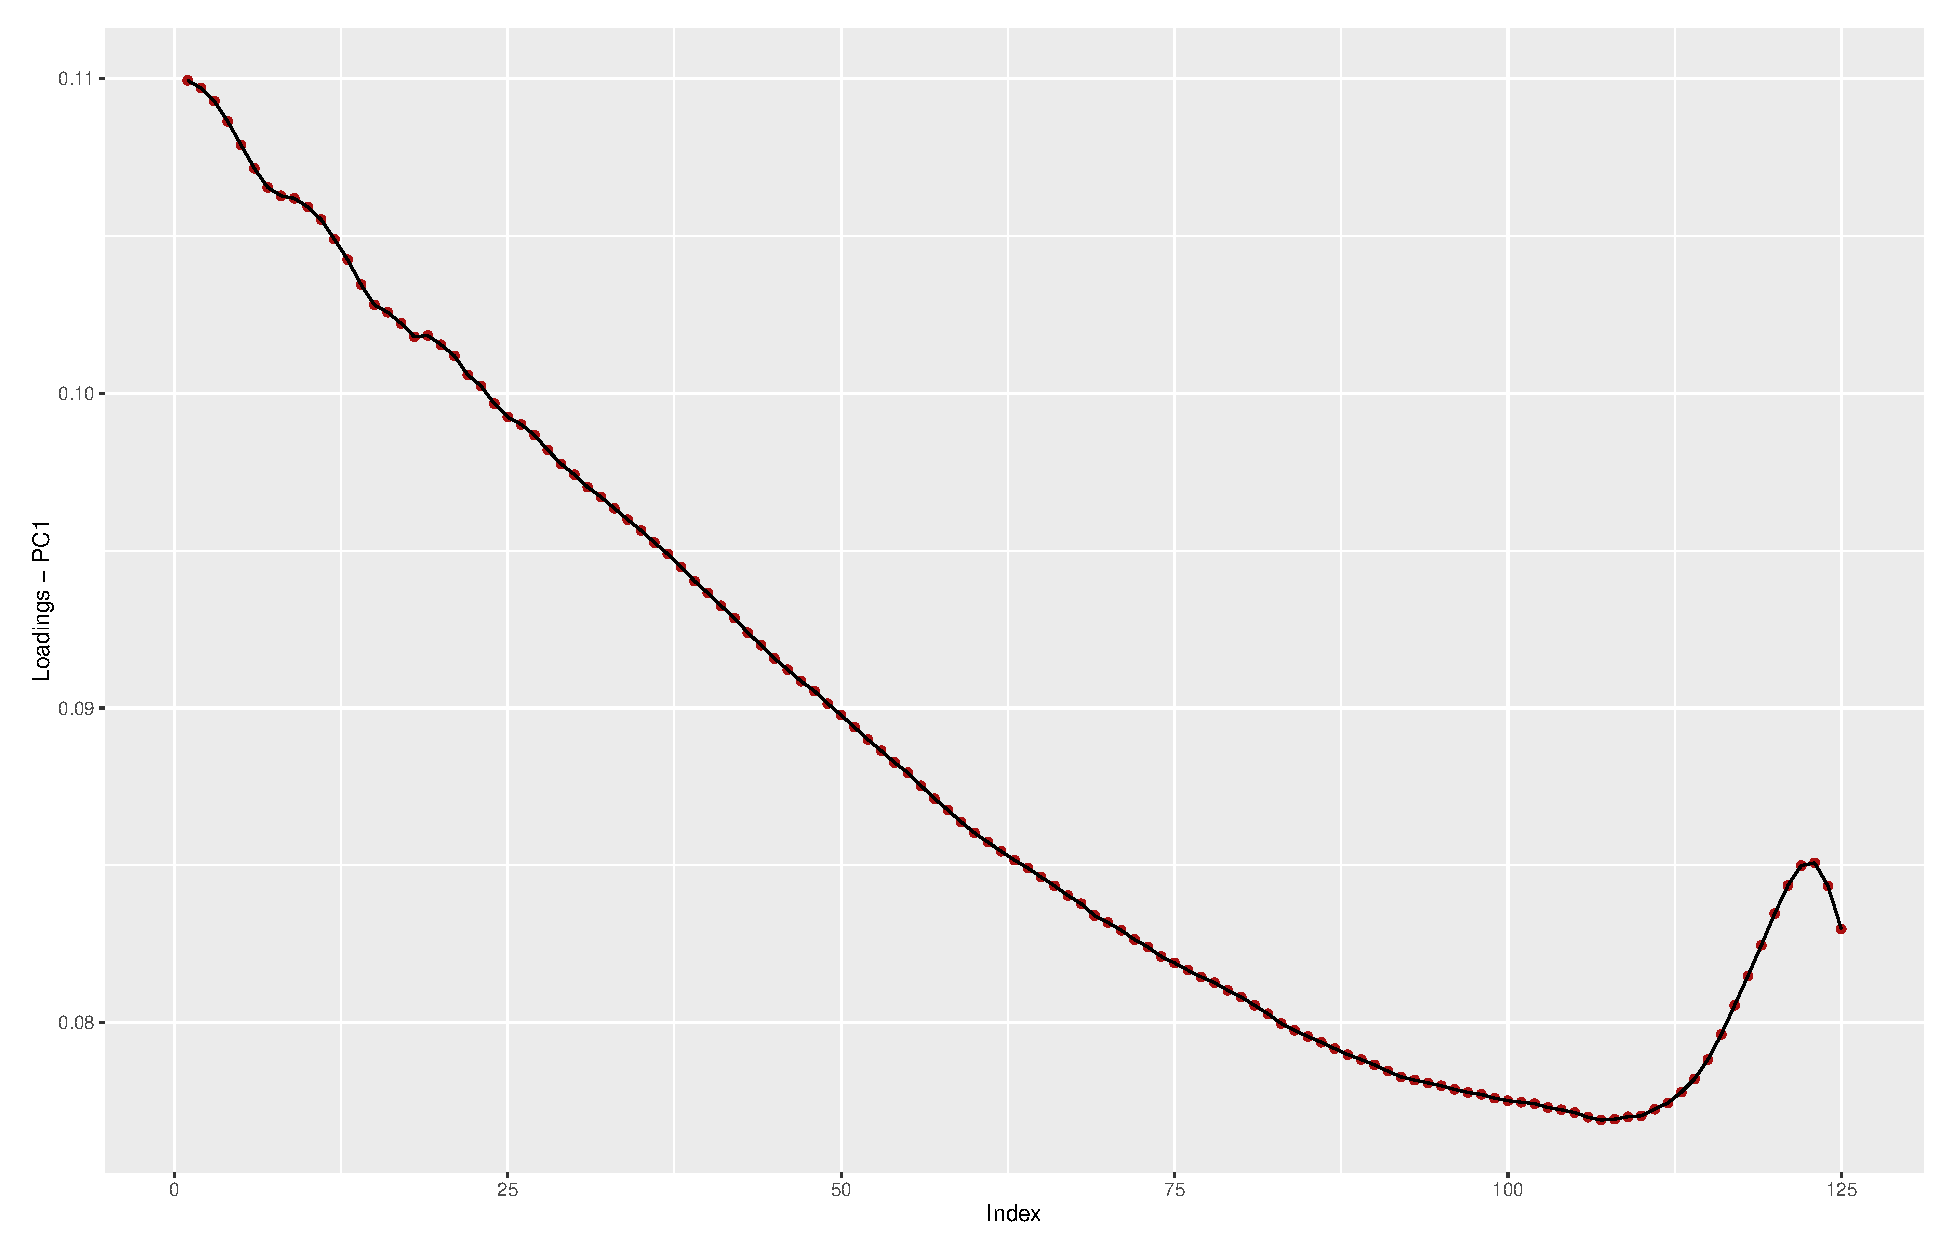
\includegraphics[width=\textwidth]{share/A2_trace_PC1.eps}
            \end{minipage}
            \begin{minipage}[]{0.49\textwidth}
                \caption{Trace plot of PC2 \label{fig:x752tp}}
                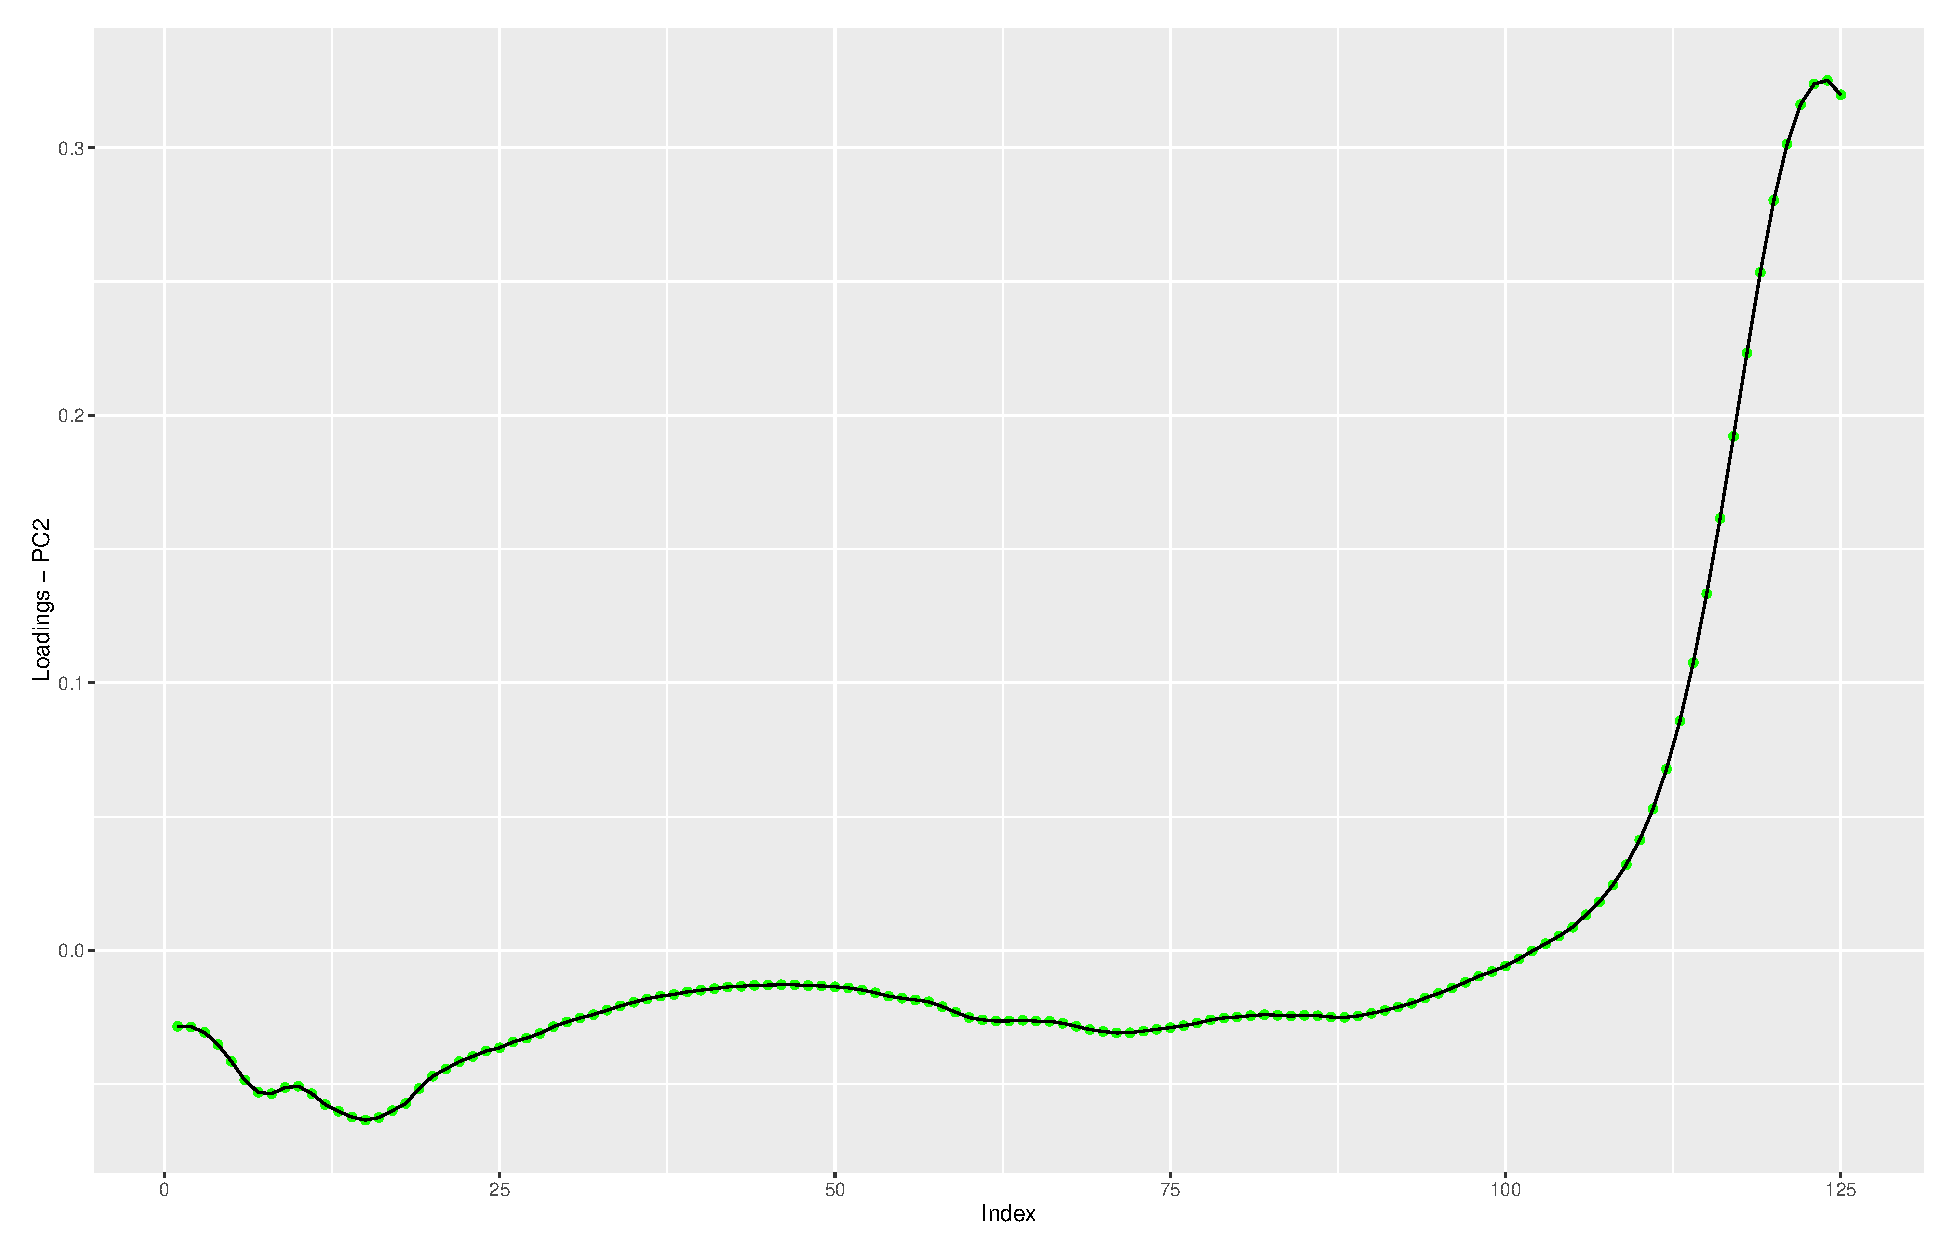
\includegraphics[width=\textwidth]{share/A2_trace_PC2.eps}
            \end{minipage}
        \end{figure}

        Note the high correlation values in the same index on both plots. High value indicates higher correlation with the selected components. There are a couple of components which are relatively highly explained by the components extracted from the previous analysis. PC1 correlates highly with the first components and PC2 with the last ones. 


    \subsection*{Independent Component Analysis}

        We perform the same analysis again, this time using the \emph{Independent component analysis} (ICA). In contrast to to PCA, where we assumed the features are correlated, we assume that they are independent. 

        The loadings are calculated with the function \( \hat{W} = K \dot W \). We plot the traces for each column (the chosen components), the result can observed in Figures~\ref{fig:x750ical}, \ref{fig:x752ical}.
        \lstinputlisting[firstline=42,lastline=45]{../share/assignment2.r}

        \begin{figure}[H]
            \centering
            \begin{minipage}[]{0.49\textwidth}
                \caption{Trace plot of IC1\label{fig:x750ical}}
                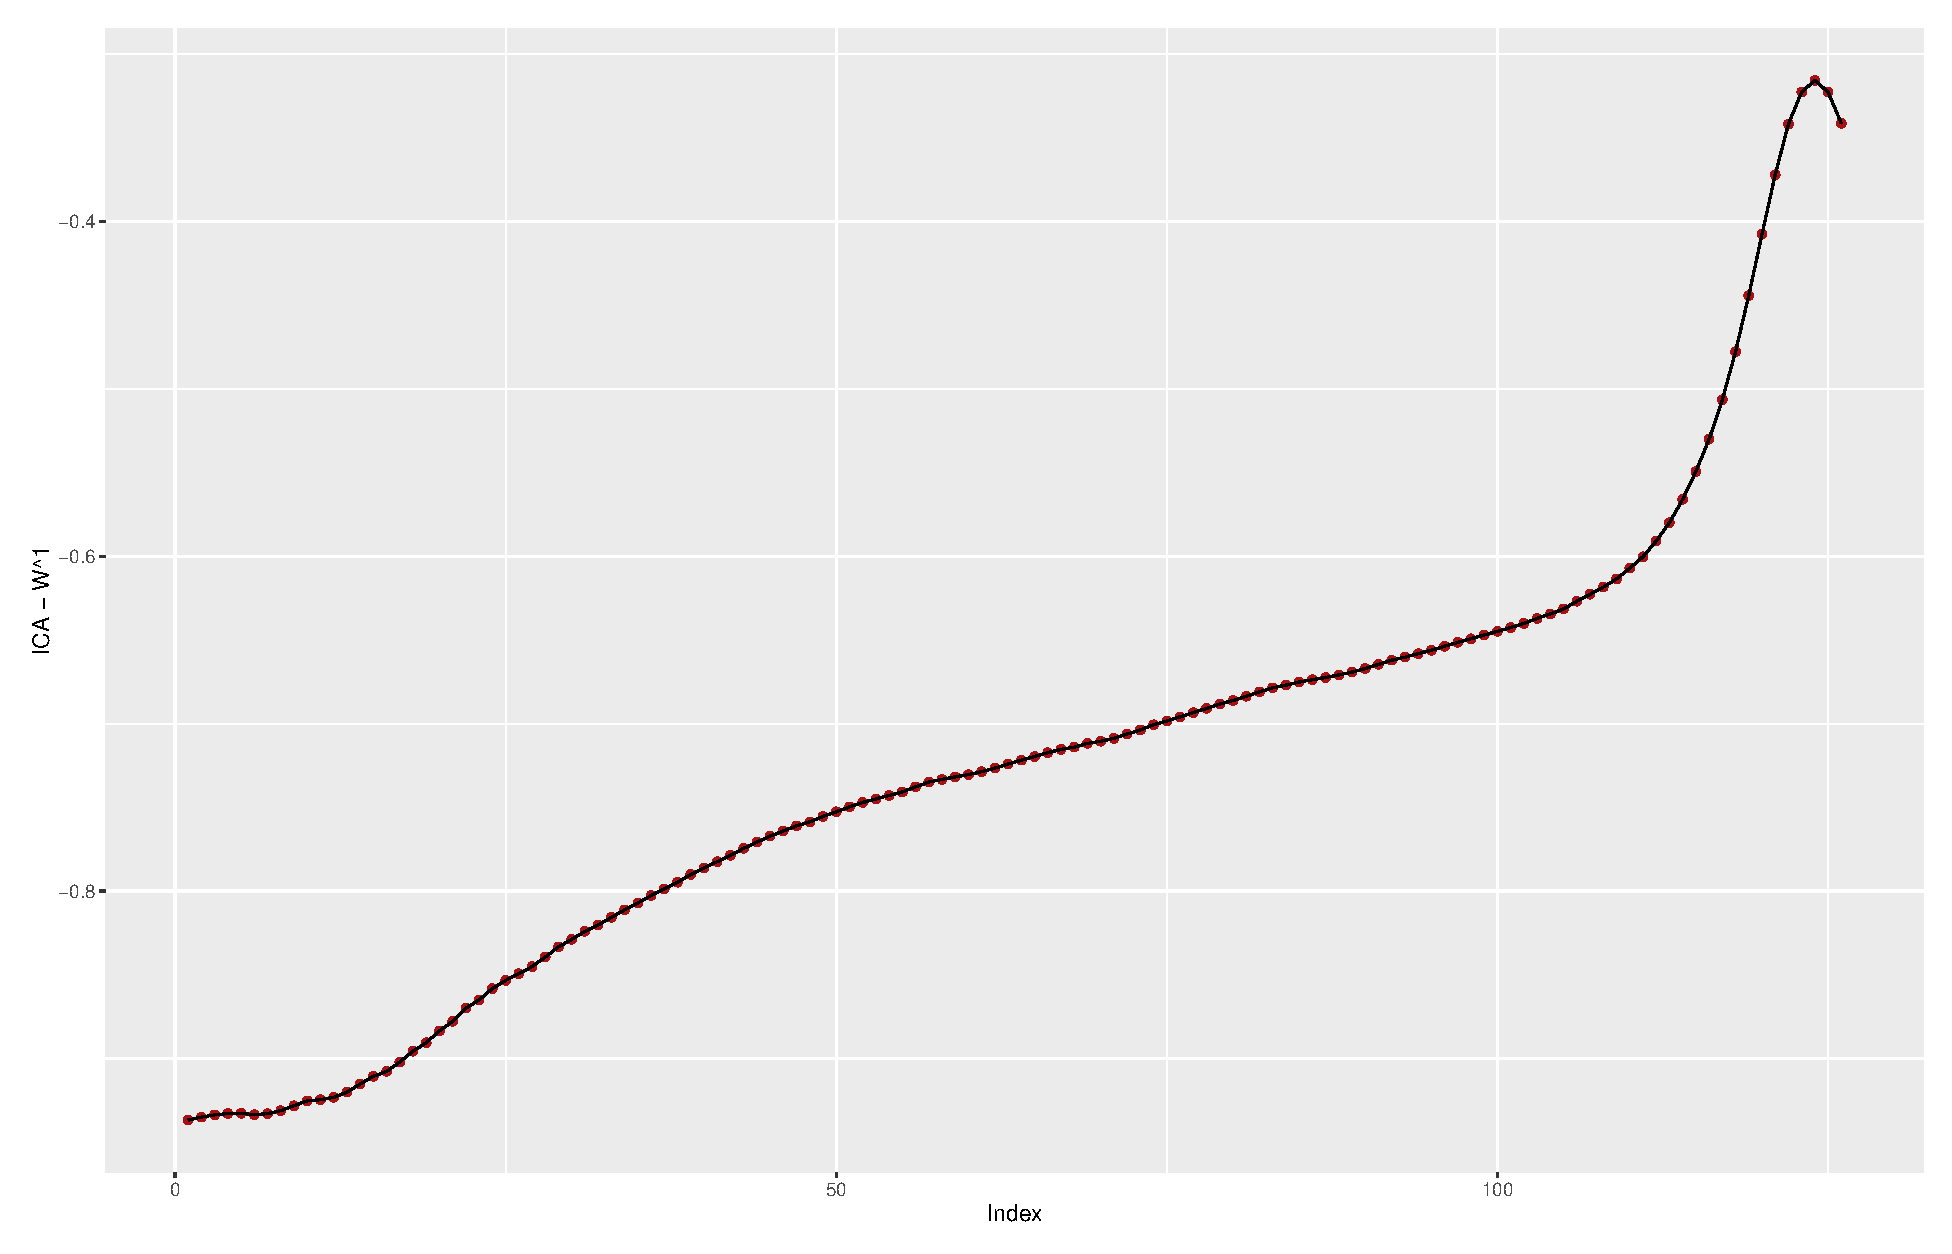
\includegraphics[width=\textwidth]{share/A2_trace_ICA1.eps}
            \end{minipage}
            \begin{minipage}[]{0.49\textwidth}
                \caption{Trace plot of IC2\label{fig:x752ical}}
                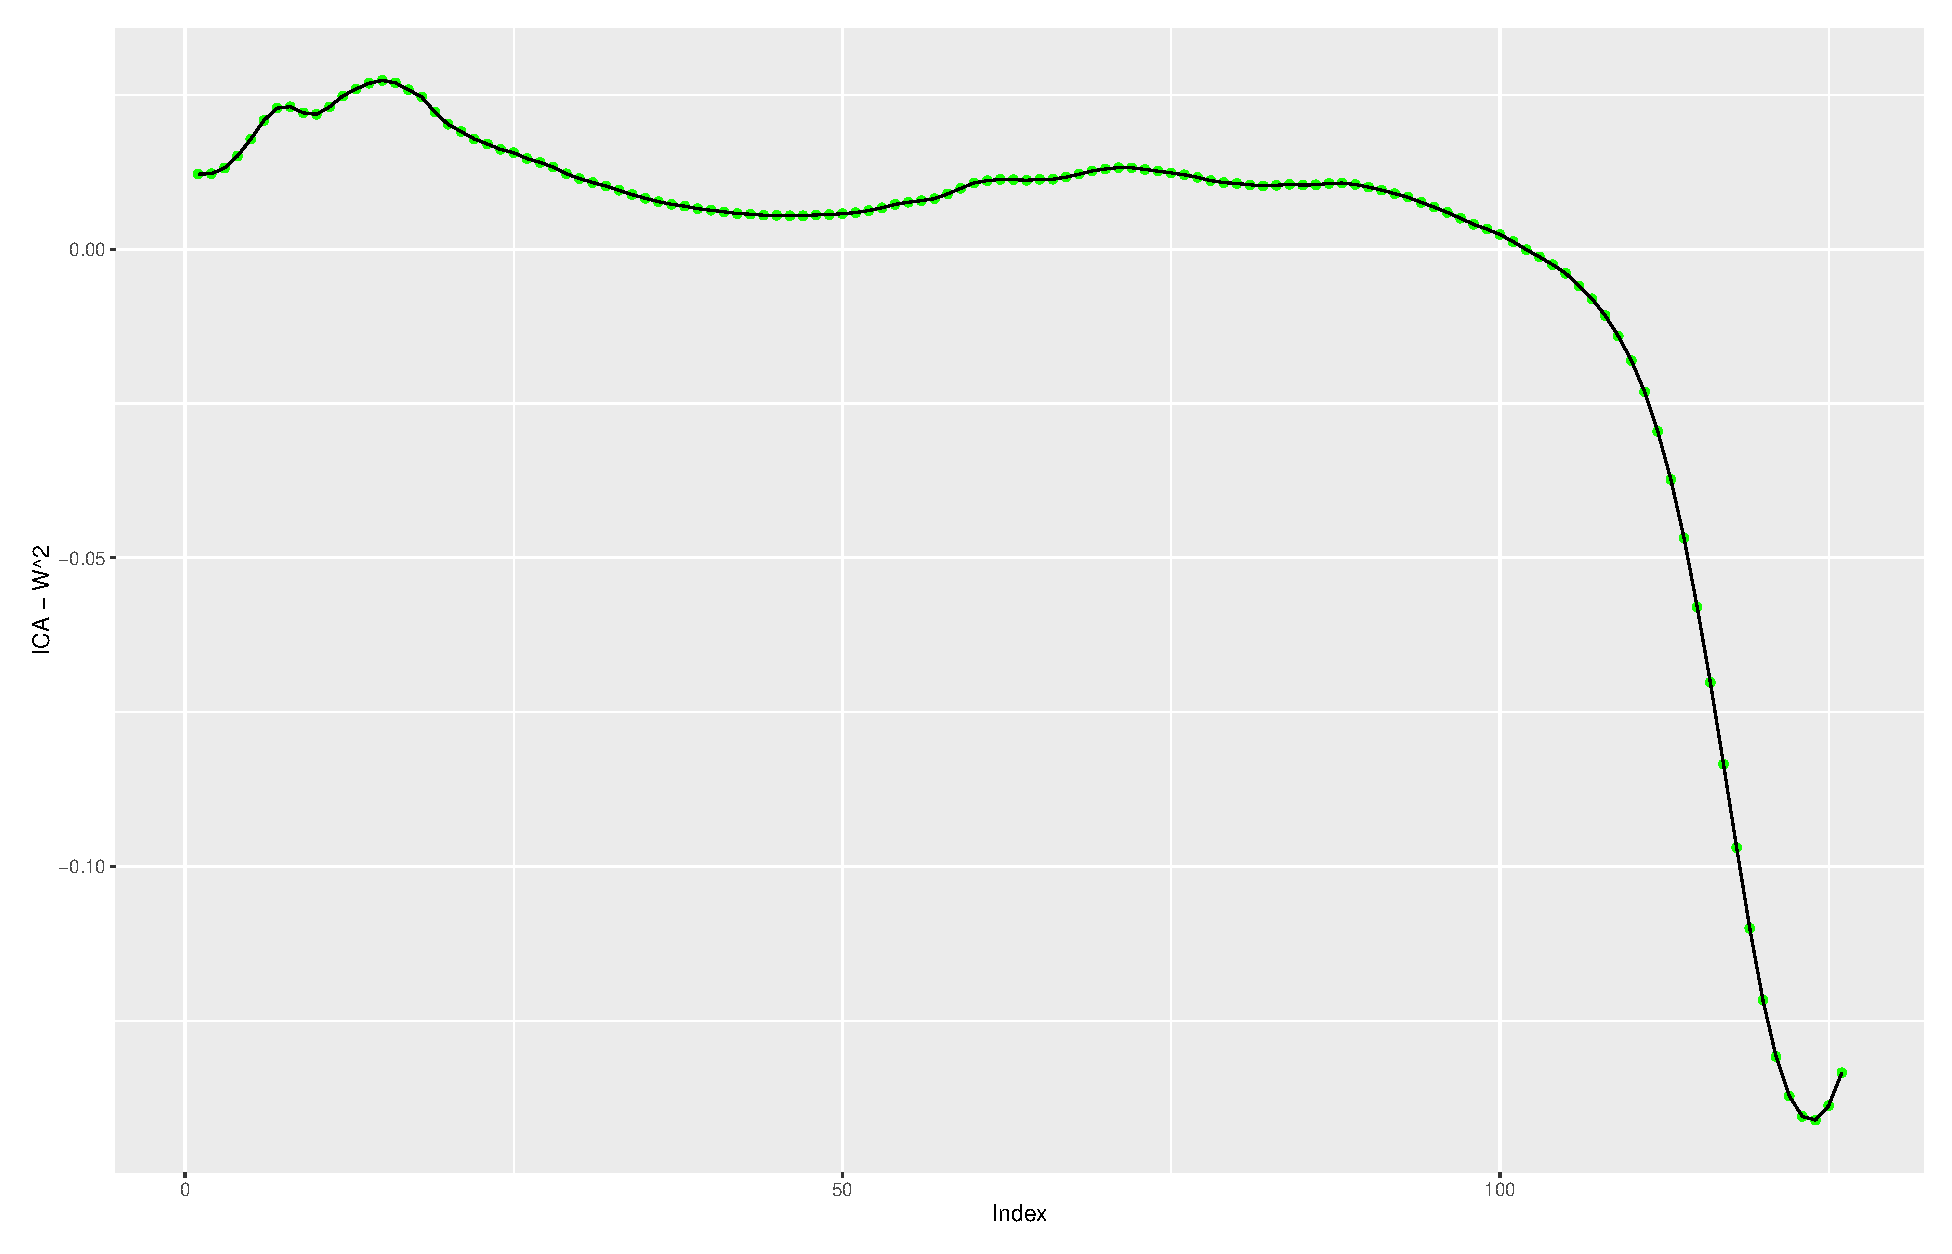
\includegraphics[width=\textwidth]{share/A2_trace_ICA2.eps}
            \end{minipage}
        \end{figure}

        The results are quite similar to those found in PCA, but inverted. Now the IC1 correlates with the last couple of components while IC2 correlates with the first ones.

        We now plot the scores found by doing ICA, which can be seen in Figure~\ref{fig:icascores}.

        \begin{figure}[H]
            \centering
            \caption{ICA score distribution}
            \label{fig:icascores}
            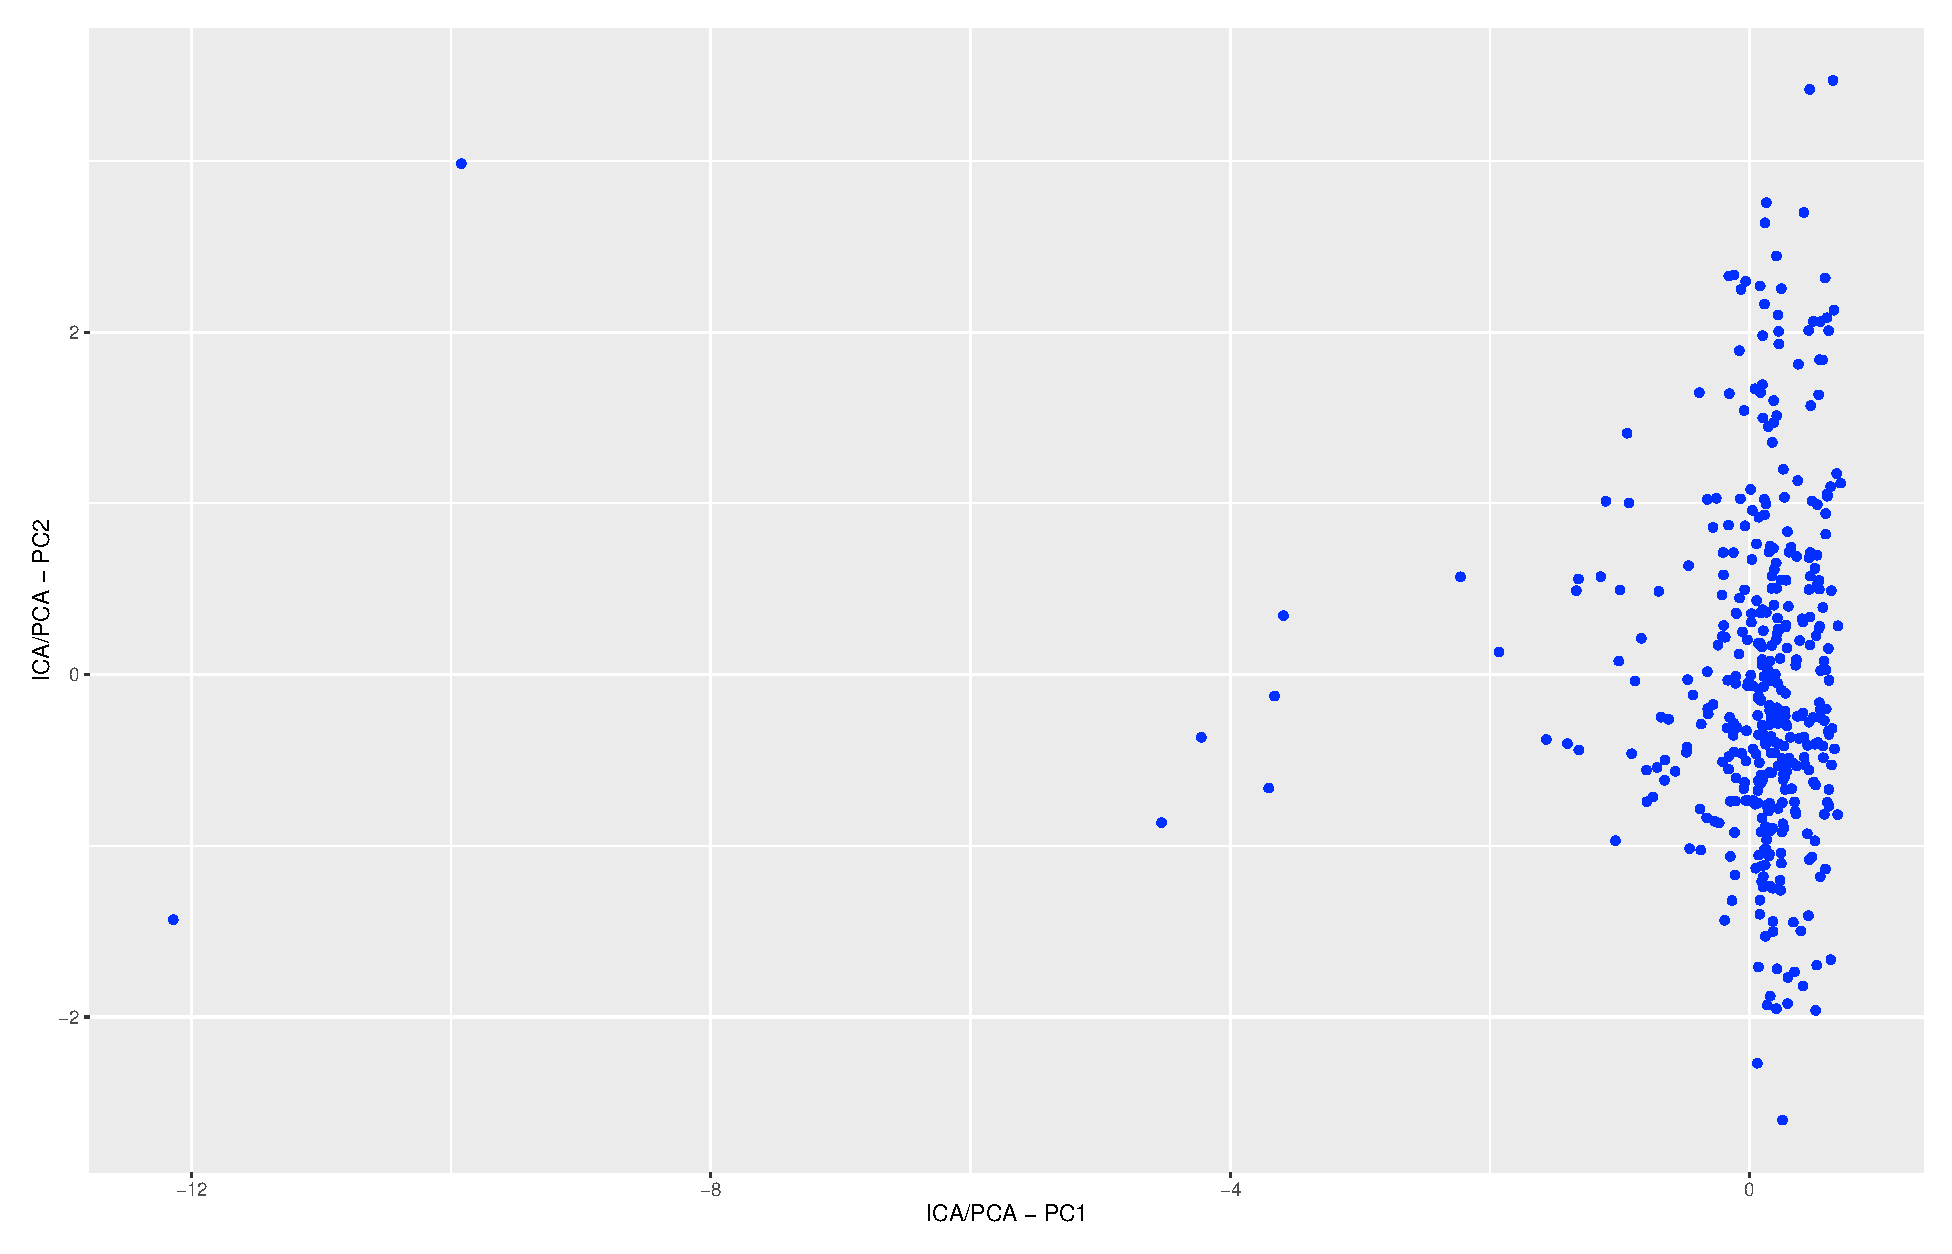
\includegraphics[width=\textwidth]{share/A2_icascore.eps}
        \end{figure}

        The score distribution has a much higher magnitude compared to PCA and the distribution is mirrored in the Y-axis. Otherwise they look very similar. The PCA score distribution can be observed in figure~\ref{fig:pcascore}.
    \subsection*{PCA Cross-Validation}

 		We perform a \emph{Principal component regression} analysis with \emph{cross validation} in order to examine the number of components that should be selected. Below is the resulting plot (\ref{fig:icascores}) of \emph{predicted mean-squared error} in relation to the number of components selected for the model.
        \lstinputlisting[firstline=66,lastline=67]{../share/assignment2.r}

        \begin{figure}[H]
            \centering
            \caption{Mean squared predicted error over number of components}
            \label{fig:viscosity}
            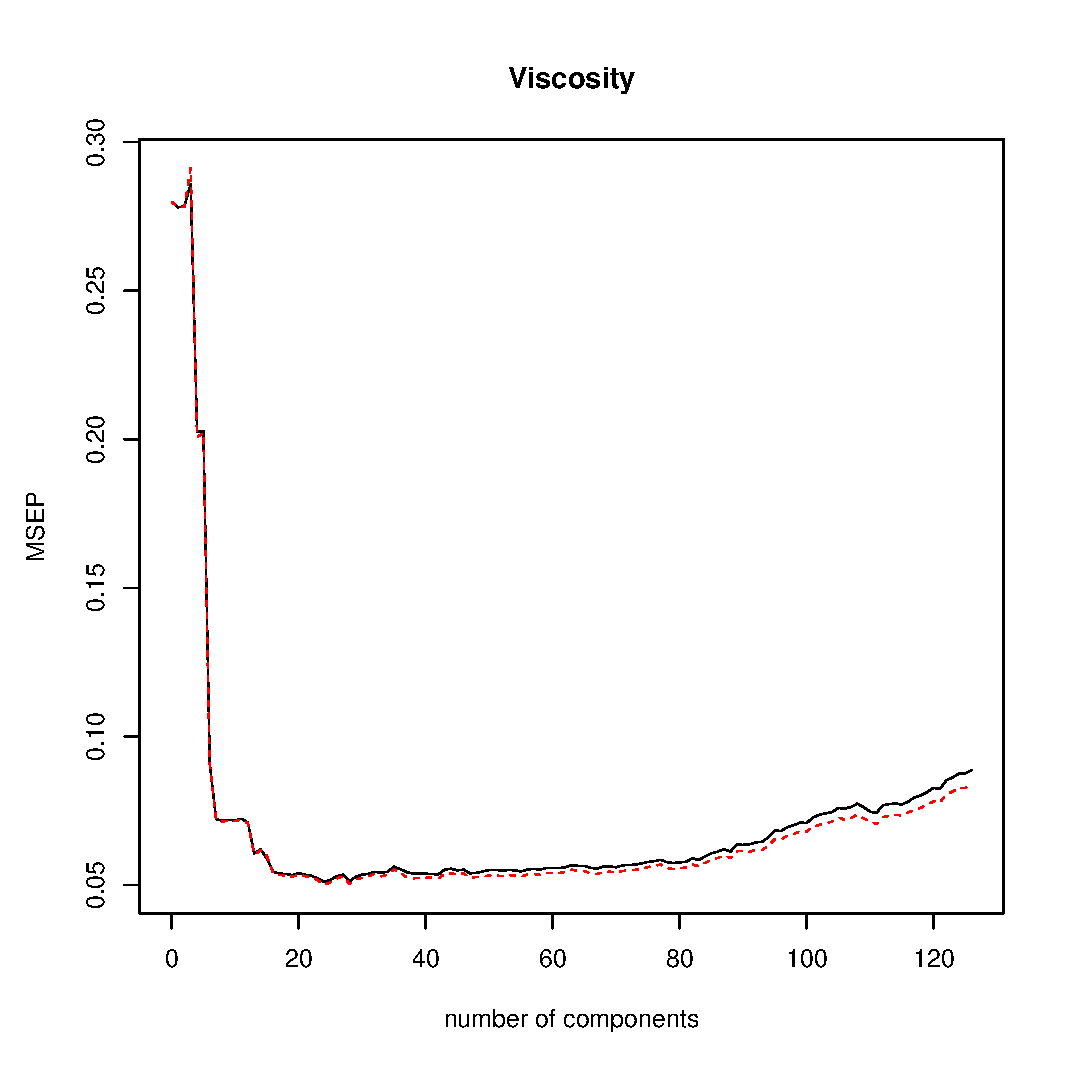
\includegraphics[width=\textwidth]{share/A2_viscosity.eps}
        \end{figure}

	We can observe from the figure how the MSEP is high when few components are selected and how the MSEP drastically decreases around 8 components. The number of components with the lowest MSEP is around 20 and after that it slowly increases. The optimal number of components appears to be around 20. 
	
    \section*{Contributions}
        Most of the text contained in this report was written in conjunction with the entire group, therefore the main body of the text is the work of everyone.
    \begin{itemize}
        \item{\textbf{Martin Estgren:} provided all the figures, the code for assignment 1, and wrote a lot of the analysis of assignment 2.}
        \item{\textbf{Erik S. V. Jansson:} provided the script for assignment 2, and polished several sections found in assignment 1.}
    \end{itemize}
    \nocite{*} % No warnings.
    \bibliographystyle{alpha}
    \bibliography{report}
    \onecolumn \appendix
    \section*{Appendix}

    \lstinputlisting[caption={Script for Assignment 1 on Bootstrapping},label={lst:assignment1}]{../share/assignment1.r}
    \lstinputlisting[caption={Script for Assignment 2 on Component Analysis},label={lst:assignment2}]{../share/assignment2.r}

\end{document}
